\documentclass{article}

\usepackage{graphicx}
\usepackage{tikz}
\usepackage{tikzsymbols}
\usetikzlibrary{calc,patterns,shapes.geometric}
\pagestyle{empty}
\usepackage[margin=0pt]{geometry}
\geometry{papersize={14in,12in}}

\def\centerarc[#1](#2)(#3:#4:#5){\draw[#1] ($(#2)+({#5*cos(#3)},{#5*sin(#3)})$) arc (#3:#4:#5);}

\begin{document}
	\begin{figure}
		\centering
		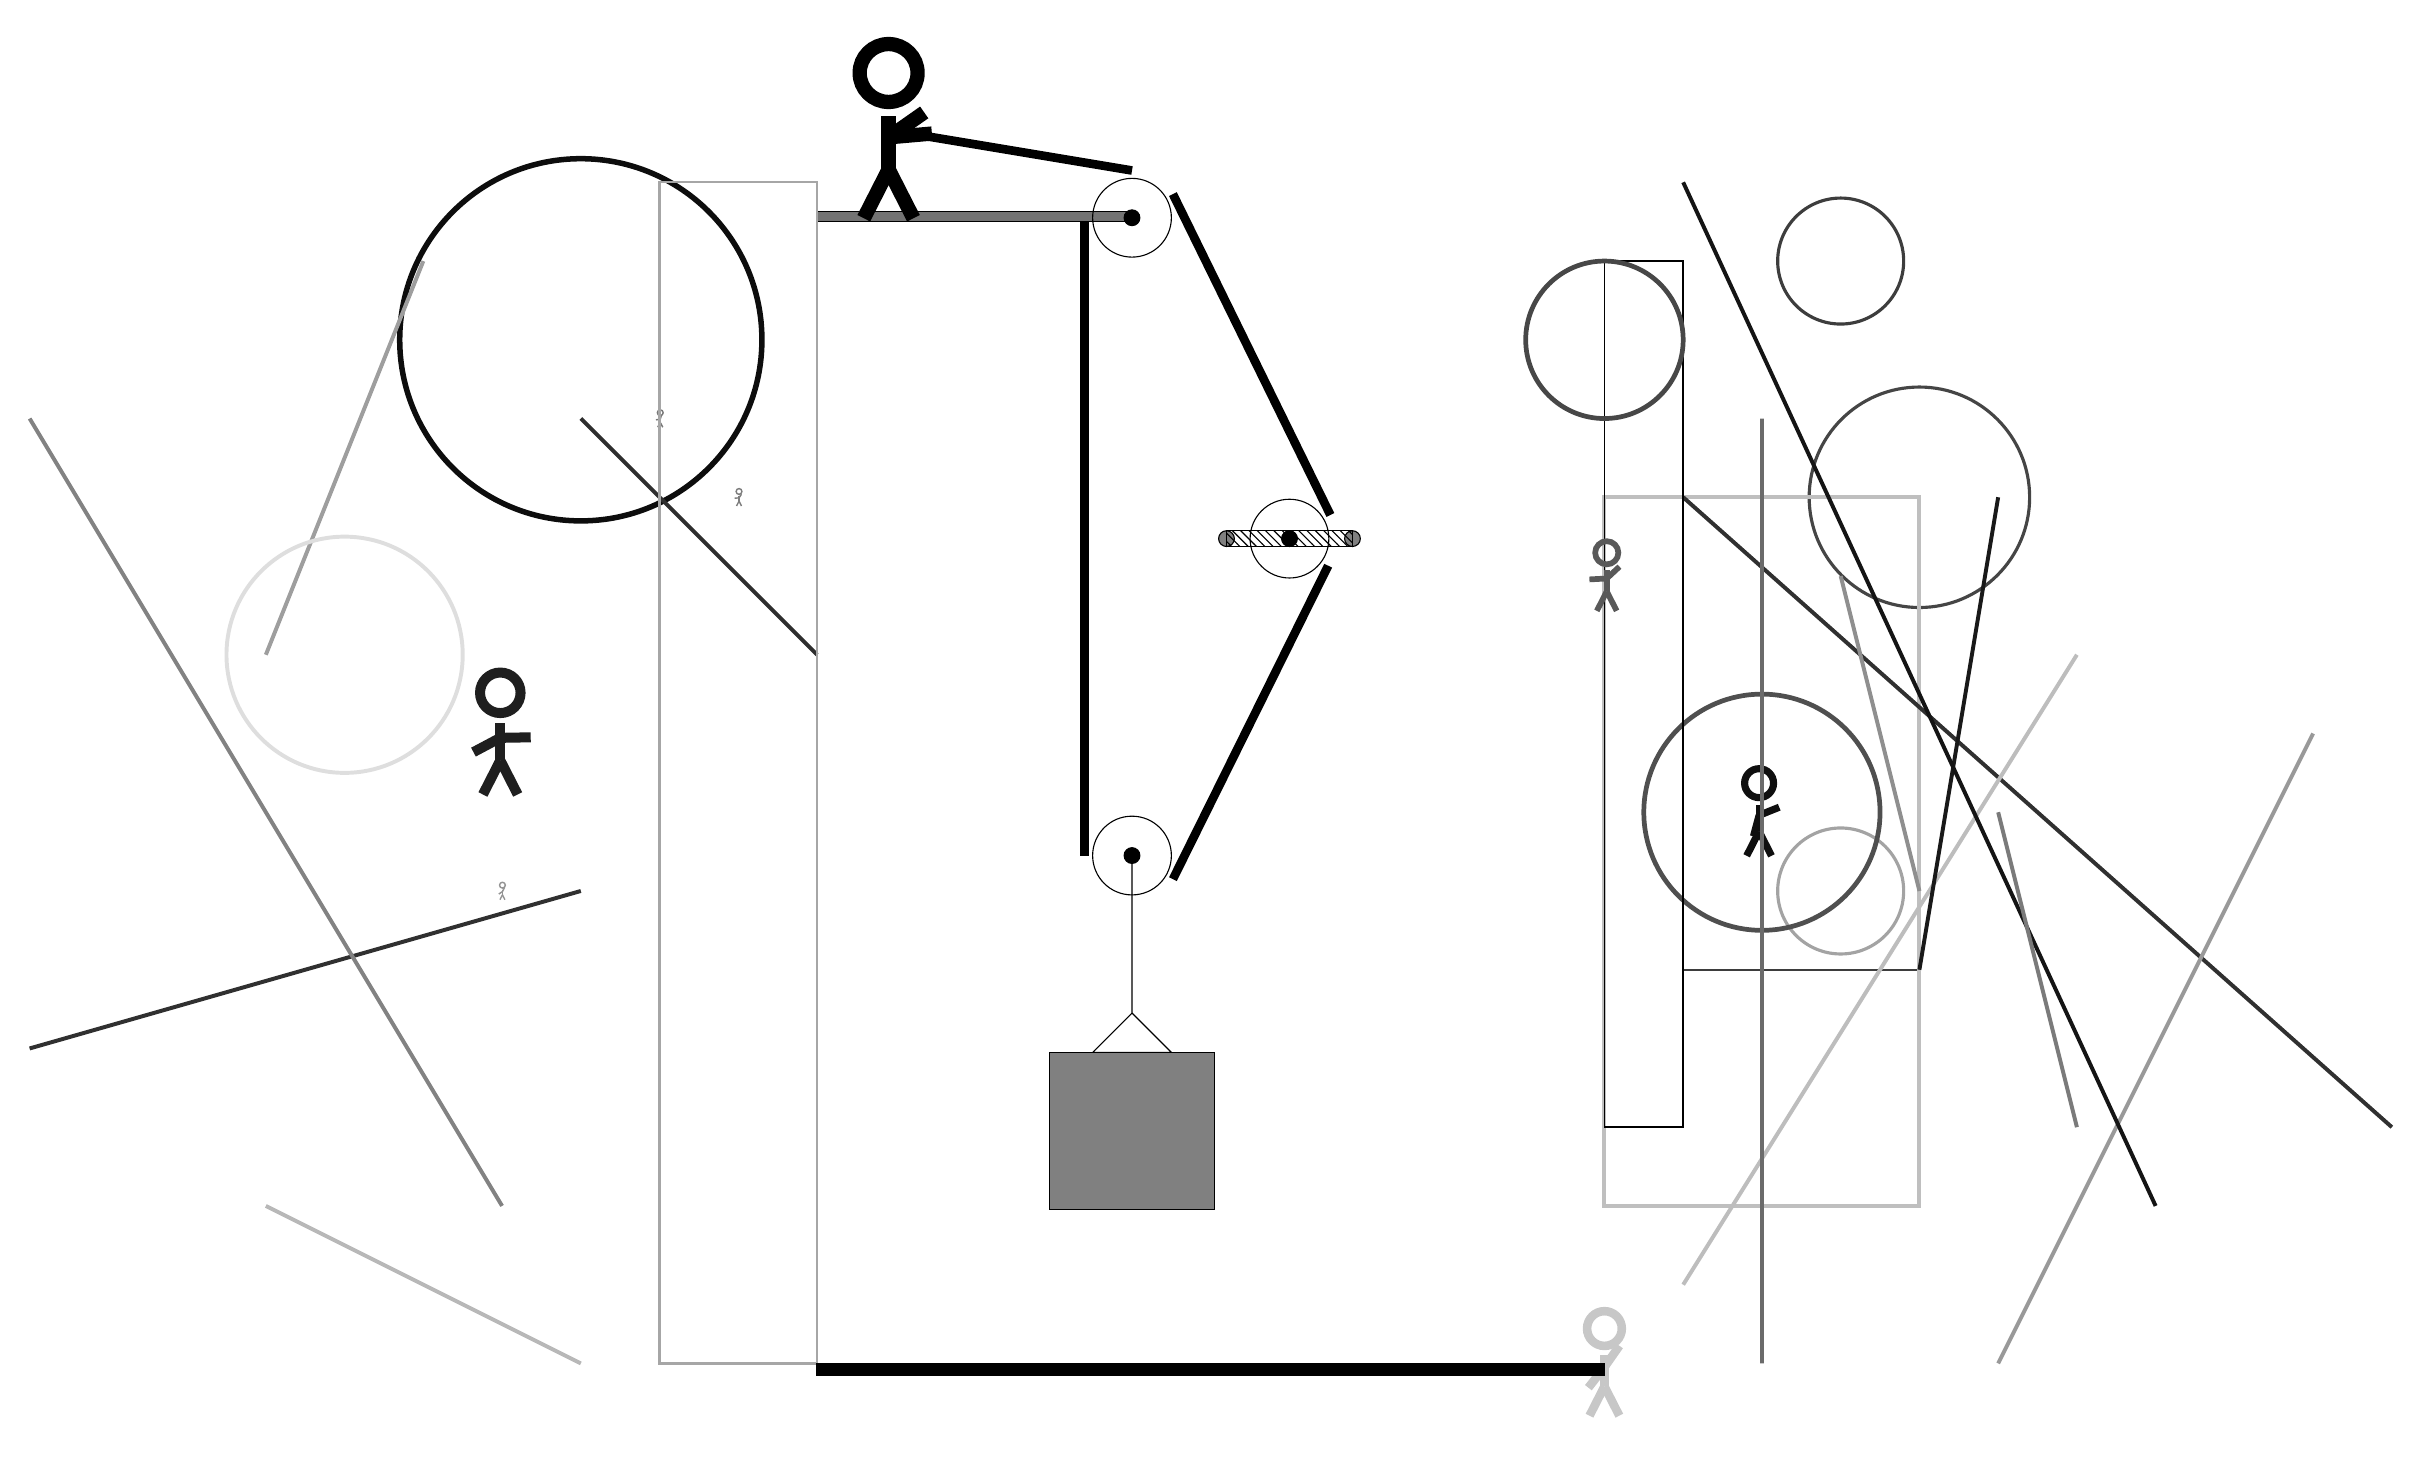
\begin{tikzpicture}
			%%%%% START %%%%%
			
			\draw[fill=black!55] (-2, 11.5) rectangle (2, 11.625);
			
			\draw (2, 3.45) circle (0.5);
			\draw[fill=black] (2, 3.45) circle (0.1);
			
			\draw (2, 11.55) circle (0.5);
			\draw[fill=black] (2, 11.55) circle (0.1);
			
			\draw[fill=white](4, 7.475) circle (0.5);
			\draw[fill=black] (4, 7.475) circle (0.1);
			\draw[fill=black!50] (3.2, 7.475) circle (0.1);
			\draw[fill=black!50] (4.8, 7.475) circle (0.1);
			\draw[pattern=north west lines, pattern color=black] (3.2, 7.575) rectangle (4.8, 7.375);
			
			\draw (2, 3.45) -- (2, 1.45) -- (1.5, 0.95) -- (2.5, 0.95) -- (2, 1.45);
			\draw[fill=black!50] (0.95, 0.95) rectangle (3.05, -1.05);
			
			\draw[line width=1.1mm] (1.4, 11.5) -- (1.4, 3.45);
			\centerarc[line width=1.1mm](2, 3.45)(180:330:0.6);
			\draw[line width=1.1mm](2.5196, 3.15) -- (4.4915, 7.1308);
			\centerarc[line width=1.1mm](4, 7.475)(390:325:0.6);
			\draw[line width=1.1mm](4.5196, 7.775) -- (2.5196, 11.85);
			\centerarc[line width=1.1mm](2, 11.55)(30:90:0.6);
			\draw[line width=1.1mm](2, 12.15) -- (-1, 12.65);
			
			\node at (-1, 12.65) {\Strichmaxerl[10][-175][35]};
			
			\draw[line width=0.5mm, color=black!81](-5, 3) -- (-12, 1);
			
			\draw [line width=0.4mm, color=black!73](12, 8) circle (1.4);
			\draw[line width=0.2mm, color=black!76] (9, 2) rectangle (12, 2);
			\draw[line width=0.5mm, color=black!25] (8, -1) rectangle (12, 8);
			\draw[line width=0.5mm, color=black!81](9, 8) -- (18, 0);
			\node[line width=0.5mm, color=black!88] at (-6, 5) {\Strichmaxerl[7][28][1]};
			
			\node[line width=0.4mm, color=black!94] at (10, 4) {\Strichmaxerl[5][75][22]};
			\node[line width=0.3mm, color=black!53] at (-4, 9) {\Strichmaxerl[1][9][73]};
			\node[line width=0.2mm, color=black!22] at (8, -3) {\Strichmaxerl[6][52][55]};
			
			\draw [line width=0.7mm, color=black!95](-5, 10) circle (2.3);
			\draw[line width=0.5mm, color=black!82](-2, 6) -- (-5, 9);
			
			\draw [line width=0.4mm, color=black!76](11, 11) circle (0.8);
			\draw [line width=0.4mm, color=black!36](11, 3) circle (0.8);
			\draw [line width=0.6mm, color=black!69](10, 4) circle (1.5);
			\node[line width=0.4mm, color=black!51] at (-3, 8) {\Strichmaxerl[1][3][57]};
			\draw[line width=0.3mm, color=black!35] (-2, -3) rectangle (-4, 12);
			
			\draw[line width=0.5mm, color=black!40](13, -3) -- (17, 5);
			
			\draw[line width=0.2mm, color=black!100] (8, 0) rectangle (9, 11);
			\draw[line width=0.5mm, color=black!26](9, -2) -- (14, 6);
			\draw[line width=0.5mm, color=black!49](-6, -1) -- (-12, 9);
			\draw[line width=0.5mm, color=black!90](12, 2) -- (13, 8);
			
			\draw[line width=0.5mm, color=black!44](11, 7) -- (12, 3);
			\draw[line width=0.5mm, color=black!28](-5, -3) -- (-9, -1);
			\node[line width=0.2mm, color=black!65] at (8, 7) {\Strichmaxerl[4][3][43]};
			\draw [line width=0.6mm, color=black!72](8, 10) circle (1.0);
			
			\draw[line width=0.5mm, color=black!58] (10, 9) rectangle (10, -3);
			\draw[line width=0.5mm, color=black!92](9, 12) -- (15, -1);
			\draw[line width=0.5mm, color=black!38](-7, 11) -- (-9, 6);
			\node[line width=0.2mm, color=black!42] at (-6, 3) {\Strichmaxerl[1][34][63]};
			\draw[line width=0.5mm, color=black!52](13, 4) -- (14, 0);
			\draw [line width=0.5mm, color=black!13](-8, 6) circle (1.5);
			
			\draw[fill=black] (-2, -3) rectangle (8, -3.15);
			
			%%%%% END %%%%%
		\end{tikzpicture}
	\end{figure}	
\end{document}